\documentclass{article}

\usepackage{amsmath}
\usepackage{fancyhdr}
\usepackage{graphicx}
\graphicspath{{}}

%% some colours
\usepackage{color}
\definecolor{deepblue}{rgb}{0,0,0.5}
\definecolor{deepred}{rgb}{0.6,0,0}
\definecolor{deepgreen}{rgb}{0,0.5,0}
\definecolor{backcolour}{rgb}{0.95,0.96,0.93}

%%%%%%%%%%%%%% CODE STUFF %%%%%%%%%%%%%%
%%%%%%%%%%%%%%%%%%%%%%%%%%%%%%%%%%%%%%%%
\usepackage{cprotect} % to be used in sol
\usepackage{listings} % for code display
% setting code style
\newcommand\pythonstyle{\lstset{
        language=Python,
        backgroundcolor=\color{backcolour},
		basicstyle=\footnotesize,
		otherkeywords={self},
		keywordstyle=\footnotesize\color{deepblue},
		emph={__init__},
		emphstyle=\footnotesize\color{deepred},
		stringstyle=\color{deepgreen},
		frame=single,
		showstringspaces=false  ,
		breaklines=true,
		numbers=left,
		numberstyle=\footnotesize,
		tabsize=4,
		breakatwhitespace=false
	}}

% Python environment
\lstnewenvironment{python}[1][]{
    \pythonstyle
    \lstset{#1}
}{}

% Python for external files
\newcommand\pythonexternal[2][]{{
    \pythonstyle
    \lstinputlisting[#1]{#2}
}}

% Python for inline
\newcommand\pythoninline[1]{{\pythonstyle\lstinline!#1!}}

%%%%%%%%%%%%%%%%%%%%%%%%%%%%%%%%%%%%%%%%
% setting the style for ex documents
\pagestyle{fancy}
\fancyhf{}
\fancyhead[L]{\thetitle}
\fancyhead[C]{}
\fancyhead[R]{\theauthor}
\renewcommand{\headrulewidth}{0.4pt} %obere Trennlinie
\fancyfoot[L]{Due: \thedate}
\fancyfoot[R]{\thepage} %Seitennummer
\renewcommand{\footrulewidth}{0.4pt}

% include solutions
\newcommand\sol[1]{{\large\textbf{\\Solution:}}#1}


\title{BPP Exercise 4 - Lists and Collections}
\author{A. Hain, M. Nipshagen}
\date{30.04.2018, 8:00}

\makeatletter
\let\thetitle\@title
\let\theauthor\@author
\let\thedate\@date
\makeatother

% do not include solutions
\renewcommand\sol[1]{}

\begin{document}

The deadline for this exercise sheet is \textbf{Monday, \thedate.}
%
%\section*{Introductory Words}
%In case we have some information that doesn't directly concern the current exercises.
%
\section{Vector Math}
We can model vectors with tuples and lists. Python however is not equipped with the tools to do vector math, but we can write the functions for this ourselves!\\
Write a script \texttt{vectors.py} which defines the following functions:
\begin{itemize}
  \item \texttt{add(x, y)}: Adds $x$ and $y$ such that the result follows $z_i = x_i + y_i$.
  \item \texttt{sub(x, y)}: Subtracts $y$ from $x$ such that the result follows $z_i = x_i - y_i$.
  \item \texttt{dot(x, y)}: Calculates the scalar (dot) product (or inner product) of $x$ and $y$. The dot product $<x,y>$ is defined as $<x,y> = \sum\limits_{i=1}^{N}x_iy_i$.
  \item \texttt{angle(x, y)}: Calculates the angle between the between $x$ and $y$. The angle can be found by using an alternative definition of the dot product: $<x,y> = \|x\|\|y|\ \cos\theta$, which we can solve for $\theta$ and we get $\theta = \arccos\dfrac{<x,y>}{\|x|\|y\|}$.\\
  \emph{Note:} $\|x\|$ where $x$ is a vector is called the vector norm and is calculated by $\sqrt{<x,x>}$.
  \item \texttt{pdist(x, y, **kwargs)}: The distance between the two points $x$ and $y$. Your \textit{kwargs} should recognise the keywords \texttt{metric} and \texttt{p}. Your \texttt{metric} keyword should be able to take one of the values \texttt{'euclidean', 'minkowski', 'cityblock'}, and \texttt{p} can take any integer greater or equal to one. The distance is calculated depending on the metric and should default to \texttt{euclidean}. The distances are calculated as follows:
    \begin{itemize}
      \item \texttt{euclidean}: $d_{euclid} (x,y) = \sqrt[\uproot{2}2]{\sum\limits_{i=1}^N (x_i-y_i)^2}$.
      \item \texttt{minkowski}: $d_{minkowsky} (x,y) = \sqrt[\uproot{2}\texttt{p}]{\sum\limits_{i=1}^N (x_i-y_i)^\texttt{p}}$.
      \item \texttt{cityblock}: $d_{cityblock} (x,y) = \sum\limits_{i=1}^N \|x_i-y_i\|$\\
      (\emph{Note:} $\|x\|$ is the absolute value.)
    \end{itemize}
    See figure \ref{fig:metrics} for a nicer visualisation.\\
    Don't be afraid of this. It looks scary at first, but it is not beyond the scope of what you already learned.
  \item \textbf{BONUS:} \texttt{cross(x, y)}: calculates the cross product of two vectors. This might be a bit tricky. The cross product will yield a matrix. \Large{TODO}
\end{itemize}
You can assume that all vectors have the same size.
\begin{figure}[h]
  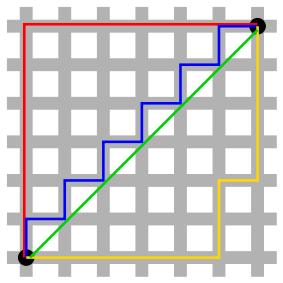
\includegraphics[scale=0.5]{metriken}
  \caption{Blue, red, and yellow are examples for the cityblock distance (it looks like following the streets of a grid city) and green is the euclidean distance.}
  \small{Taken from \url{https://en.wikipedia.org/wiki/Taxicab_geometry#/media/File:Manhattan_distance.svg}}
  \label{fig:metrics}
  
\end{figure}

\section{Which to What}
Blabla Todo, something about when to use which collection.

\section{Working together <WIP title>}
In the file \texttt{my\_collection.py} you will find two lists defined: \texttt{subjects} and \texttt{attributes}. 
In the end you should have one dictionary which uses the subject id as a key and a \textit{list} of attributes for the value.
\end{document}
